% !TeX root = main.tex

%\setkeys{Gin}{draft}
\onehalfspacing
\justifying
\par
This experiment aims to characterize an NMOS transistor for its relevant parameters, including threshold voltage ($V_{TH}$), transconductance parameter ($K$), and early voltage ($V_{A}$). The laboratory assignment utilizes Python to automate the measurement procedure and data acquisition. The ALD1106 is the device tested for this experiment.  

% Background Section
\section{Background}

Parameters $V_{TH}$, $K$, and $V_{A}$ are necessary parameters to determine both transistor bias points and small signal parameters. These parameters appear when examining the voltage-current characteristics of the NMOS transistor as follows:
\vspace{0.2cm}
\begin{itemize}
    \item \underline{Cutoff Mode:} $I_{D} = 0$ when $V_{GS} < V_{Tn}$ or $V_{DS}=0$
    
    \item \underline{Triode Mode:} $I_{D} = k_{n}^{'}\displaystyle \Bigg[\frac{W} {L}\Bigg]\Bigg(V_{OVn}-\frac{1}{2}V_{DS}\Bigg)V_{DS}$ when $V_{GS} > V_{Tn}$ \& $V_{DS}<V_{OVn}$
    
    \item \underline{Saturation Mode:} $I_{D} = K_{N}V_{OVn}^2\left(1+\displaystyle\frac{V_{DS}}{|V_{A}|}\right)$ when $V_{GS} > V_{Tn}$ \& $V_{DS}\geq V_{OVn}$ 
\end{itemize}
\vspace{0.2cm}
Typically in saturation mode, the $1+V_{DS}/|V_{A}|$ term is ignored when performing the DC analysis of a transistor circuit. However, in this lab experiment it is a critical parameter to ensure that the appropriate approximations can be made to linearize data for parameter extraction. 

\section{Experiment 1: \texorpdfstring{$I_{D}$ vs. $V_{DS}$}{ID vs. VDS}}
In this experiment, the $I_{D}$ vs. $V_{DS}$ curves will be generated by using the Rohde Schwarz NGU401 source measure unit (SMU) and the Keithley 3-channel programmable power supply. In this experiment, the SMU will simultaneously source the $V_{DS}$ voltage and measure the $I_{D}$ current in real time. The voltage $V_{GS}$ is generated by the programmable power supply as a family of curves is desired. A circuit schematic and wiring diagram are shown in Figure \ref{Ch1_fig:1}. The Python code list is under the Coding List in the Appendix. 
% \Cref{lst:Ch1List1}

\begin{figure}[ht]
    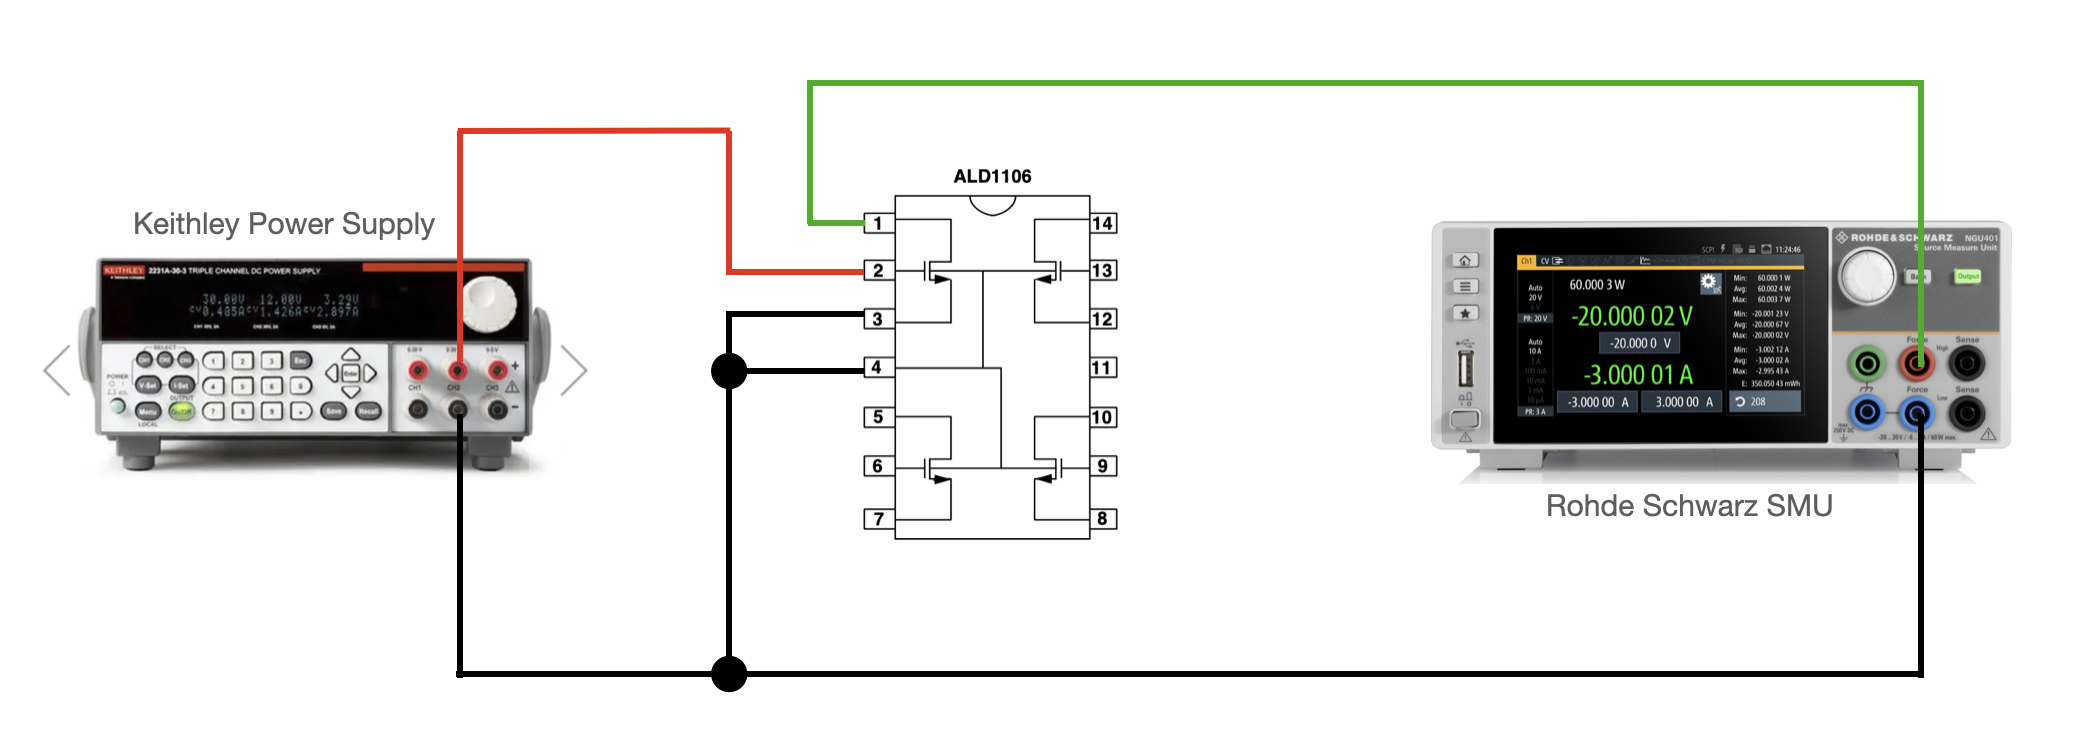
\includegraphics[scale=0.4]{graphics/Lab_01_1_1.png}
    \caption{Experiment 1 wiring diagram interfacing the transistor with the SMU and 3 channel power supply}
    \label{Ch1_fig:1}
\end{figure}

\section{Experiment 2: \texorpdfstring{$I_{D}$ vs. $V_{GS}$}{ID vs. VDS}}
In this experiment, the $I_{D}$ vs. $V_{GS}$ curves will be generated by using the Rohde Schwarz NGU401 source measure unit (SMU), the Keithley 3-channel programmable power supply and the Keithley digital multimeter (DMM). In this experiment, the SMU will source the $V_{GS}$ voltage. The voltage $V_{DS}$ is generated by the programmable power supply and the current $I_{D}$ is measured in real time by the Keithley DMM to generate the family of curves as desired. The circuit schematic remains the same; however, different voltages are being swept, therefore, the wiring diagram is modified as shown in Figure \ref{Ch1_fig:2}. The Python code list is under the Coding List~\Cref{lst:Ch1:List2}, in the Appendix. 

\begin{figure}[ht]
    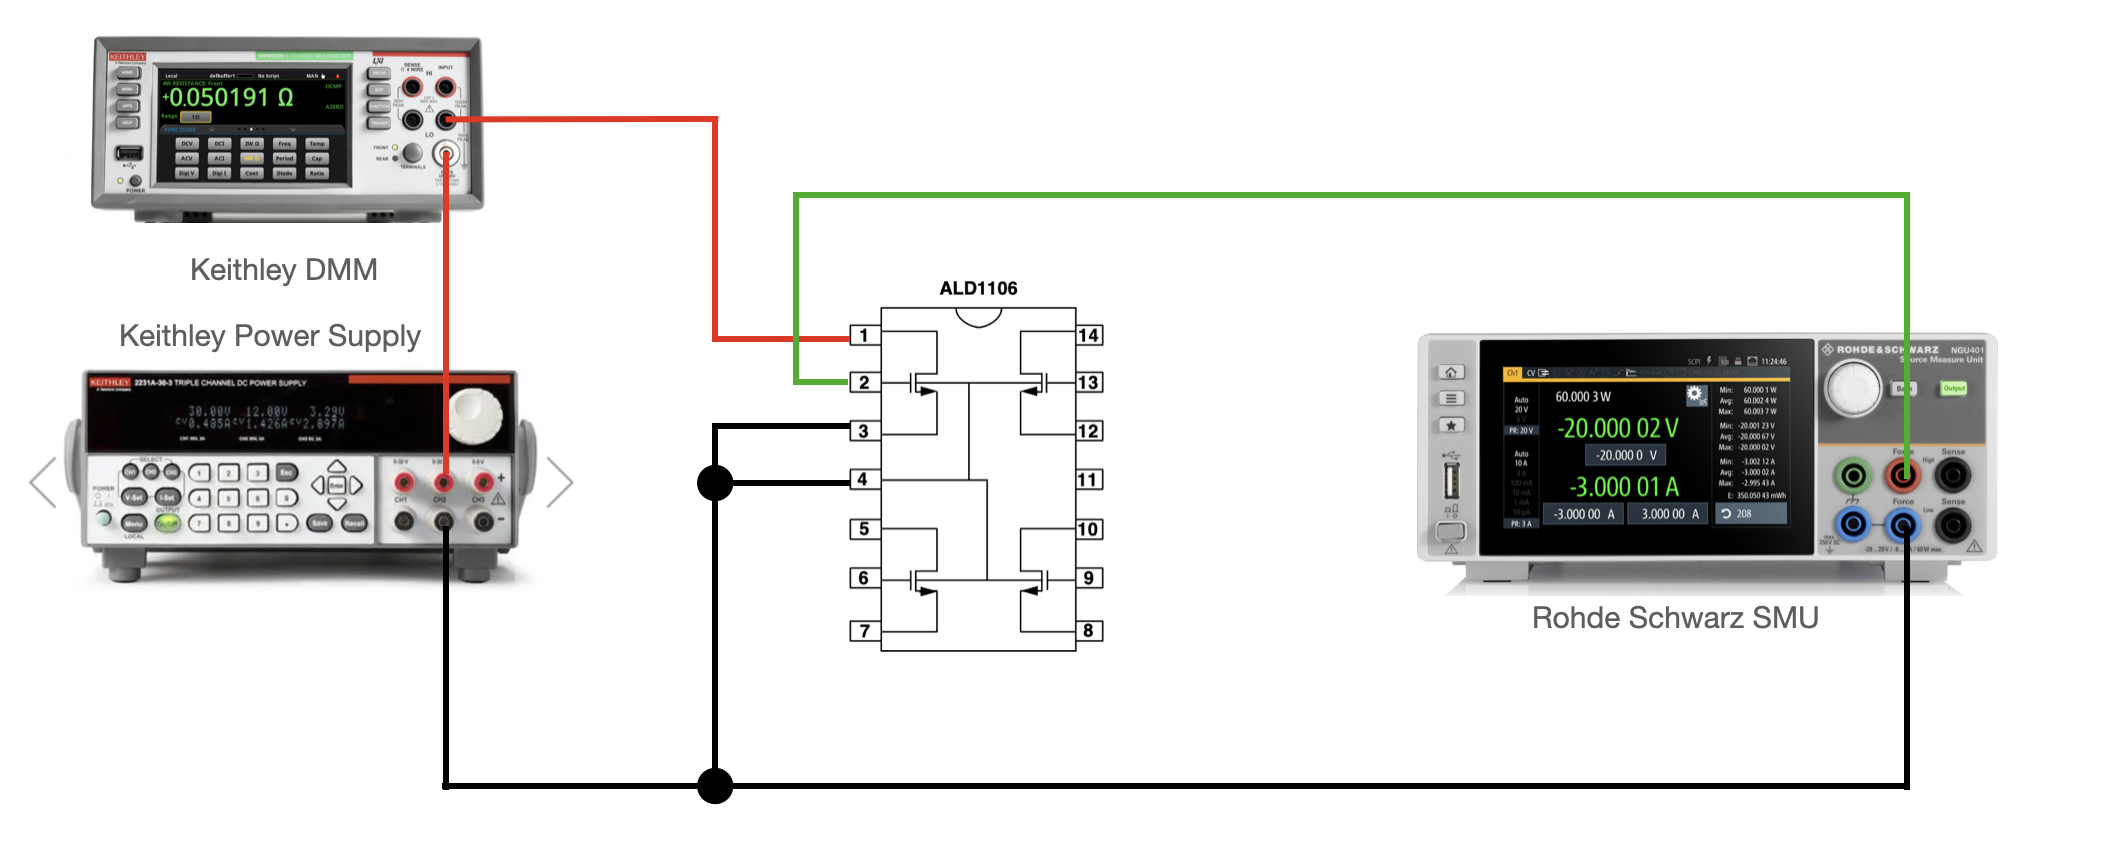
\includegraphics[scale=0.9\linewidth]{graphics/Lab_01_1_2.png}
    \caption{Experiment 2 wiring diagram interfacing the transistor with the SMU, 3 channel power supply, and digital multimeter}
    \label{Ch1_fig:2}
\end{figure}

\section{Results}
The post-laboratory tasks for this assignment included plotting the data from experiments 1 and 2. These plots include $I_{D}$ vs. $V_{DS}$ for a family of $V_{GS}$ values along with plotting $I_{D}$ vs. $V_{GS}$ for a family of $V_{DS}$ values. The transistor parameters $V_{TH}$, $K$, and $V_{A}$ are extracted by curving fitting the data from experiments 1 and 2. Code listing provides a detailed approach for the extraction of data parameters. Figure \ref{Ch1_fig:3} displays the summarized results of the experiments, and the data parameters are listed in Tables \ref{tab:1} and \ref{tab:2}.  
\cref{lst:Ch1:List3}


\begin{table}[ht]
    \centering
    \begin{tabular}{ | >{\centering\arraybackslash} m{3cm} | >{\centering\arraybackslash} m{3.5cm} |>{\centering\arraybackslash} m{5cm} | >{\centering\arraybackslash} m{2cm} | }
    \hline
    Quantity & Mean Value & Standard Deviation & Units \\
    \hline
    $K_{N}$ & 265.96 & 5.83 & $\mu$A/V \\
    \hline
    $V_{Tn}$ & 0.547 & 0.007 & V \\
    \hline

    \end{tabular}

    \caption{Summary of $\sqrt{I_{D}}$ vs. $V_{GS}$ extracted parameter values}

    \label{tab:1}
	
\end{table}

\begin{table}[ht]
\centering
\begin{tabular}{ | >{\centering\arraybackslash} m{5cm} |>{\centering\arraybackslash} m{4cm} | >{\centering\arraybackslash} m{2cm} | }
\hline
Quantity & Value & Units \\
\hline
$V_{A}$ $(V_{GS}=2$V) & -62.74 & V \\
\hline
$V_{A}$ $(V_{GS}=4$V) & -88.63 & V \\
\hline
$V_{A}$ $(V_{GS}=6$V) & -140.18 & V \\
\hline
\end{tabular}
\caption{Summary of $I_{D}$ vs. $V_{DS}$ extracted parameter values}
\label{tab:2}
\end{table}




\begin{figure}[ht]
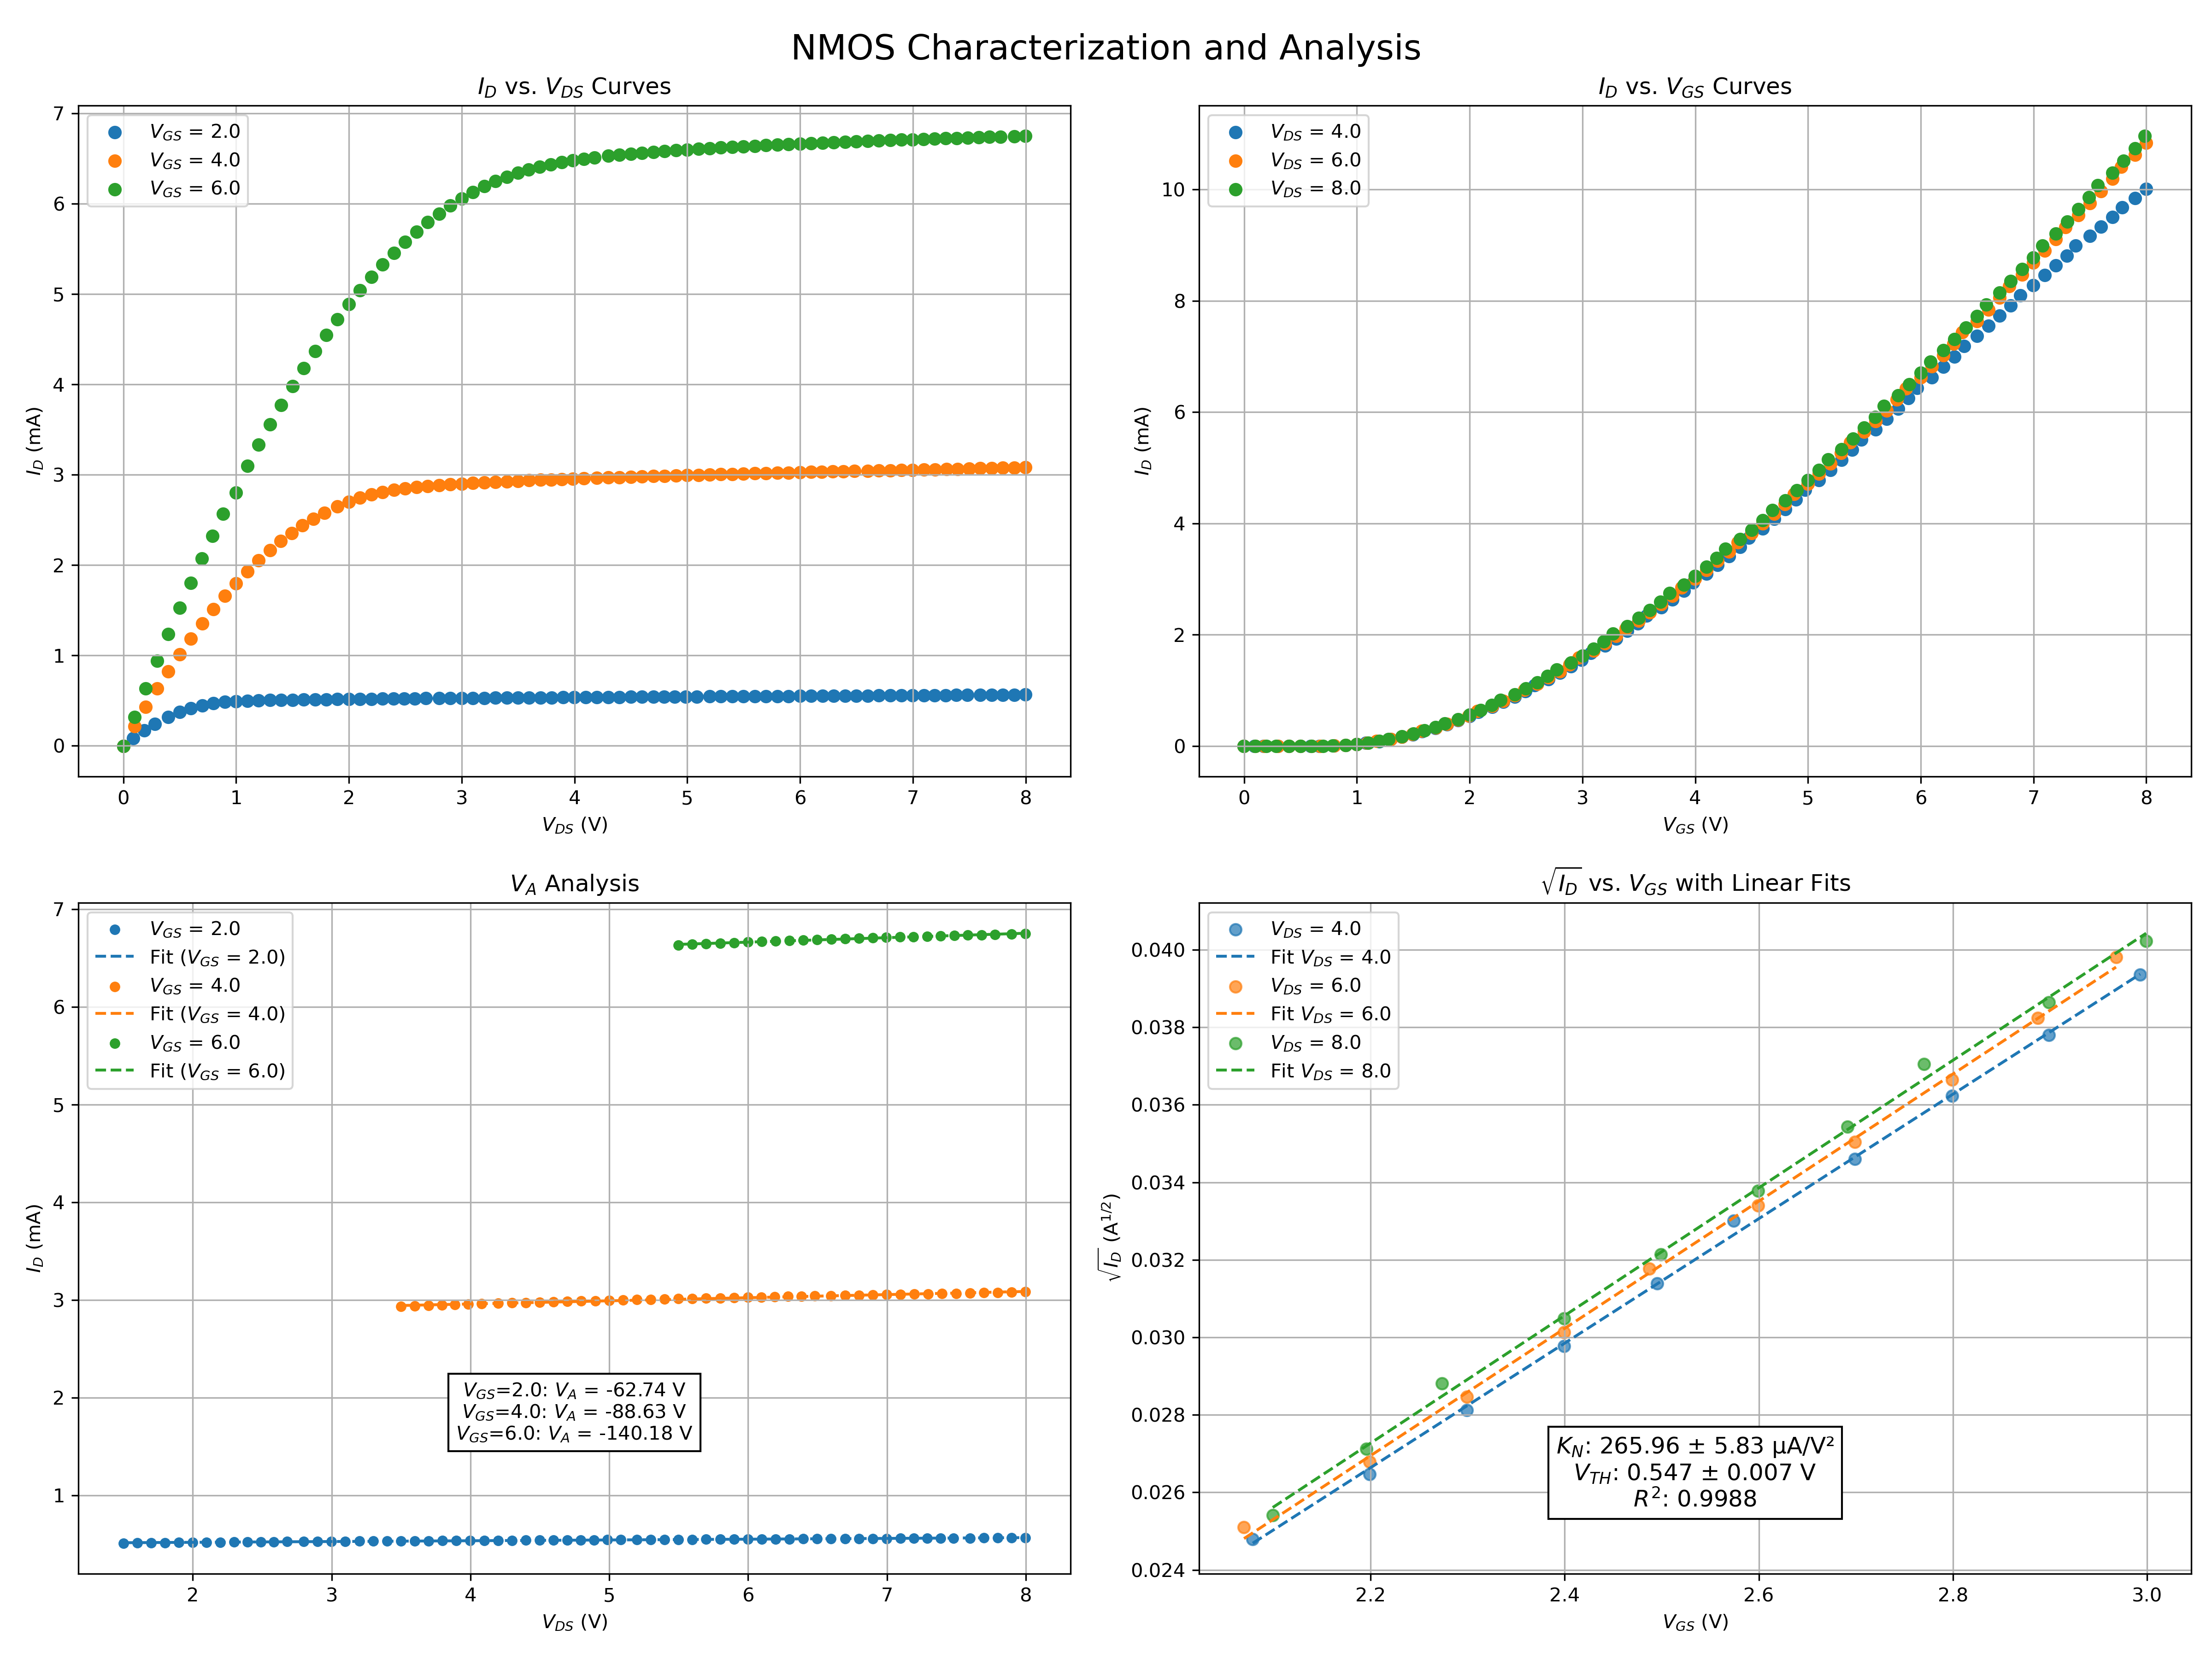
\includegraphics[scale=0.15]{graphics/Lab_01_1_3.png}
\caption{Summary of data for the NMOS characterization laboratory assignment}
\label{Ch1_fig:3}
\end{figure}

\section{Conclusions}
The data results indicate the NMOS transistor has a threshold voltage $V_{TH}$ = $0.547$, $K_{N}$ $=$ $265.96$ $\mu $ $A/V$, and Early voltages of $-62.75$, $-88.63$, and $-140.18$. The linearized region used to extract $V_{TH}$ \& $K_{N}$ had a coefficient of determination fit of $R^{2}$ $=$ $0.9988$ representing a near ideal fit across multiple data points with a small standard deviation among the various values of $V_{DS}$. The data points are chosen to minimize short channel effects from the measured results. In addition, it is experimentally observed that the Early voltage for each $V_{GS}$ sweep does not intersect the x-axis at the same point, indicating that the channel length modulation parameter is dependent on bias conditions. Therefore, when modeling this phenomenon, it likely requires a mathematical fit to fully caption its effects.